\documentclass{article}
\setlength{\parskip}{5pt} % esp. entre parrafos
\setlength{\parindent}{0pt} % esp. al inicio de un parrafo
\usepackage{amsmath} % mates
\usepackage{listings}
\usepackage[sort&compress,numbers]{natbib} % referencias
\usepackage{url} % que las URLs se vean lindos
\usepackage[top=25mm,left=20mm,right=20mm,bottom=25mm]{geometry} % margenes
\usepackage{hyperref} % ligas de URLs
\usepackage{graphicx} % poner figuras
\usepackage[spanish]{babel} % otros idiomas
\usepackage{textcomp}
\usepackage{pgfplots} % crear graficas
\pgfplotsset{width=9cm,compat=1.7}
\title{"P2" Autómata Celular} %Título
\author{NESTOR}
\date{Febrero 2022}

\begin{document} % inicia contenido

\maketitle % cabecera
\section{Introducción}


{Un autómata celular es una colección de celdas coloreadas en una cuadrícula de forma específica que evoluciona a través de una serie de pasos de tiempo discretos de acuerdo con un conjunto de reglas basadas en los estados de las celdas vecinas. Luego, las reglas se aplican iterativamente durante tantos pasos de tiempo como se desee. Von Neumann fue una de las primeras personas en considerar tal modelo e incorporó un modelo celular. Wolfram realizó estudios exhaustivos de autómatas celulares a partir de la década de 1980, y la investigación fundamental de Wolfram en el campo culminó con la publicación de su libro A New Kind of Science (Wolfram 2002) en el que Wolfram presenta una colección gigantesca de resultados relacionados con autómatas, entre los que se encuentran una serie de nuevos descubrimientos innovadores \cite{steve2}


\section{Objetivo}
El objetivo de esta práctica es examinar de manera sistemática con autómatas celulares en dos dimensiones, particularmente el famoso juego de la vida. El estado del autómata se representa con una matríz booleana (es decir, contiene ceros y unos). Cada celda es o viva (uno) o muerta (cero). En los extremos de la matríz, las celdas simplemente tienen menos vecinos. Otra alternativa sería considerar el espacio como un torus pareciendo una dona donde el extremo de abajo se reune con el extremo de arriba igual como los lados izquiero y derecho uno con otro \cite{elisa1}.

\section{Desarrollo} % seccion y etiqueta

La regla de supervivencia es sencilla: una celda está viva si exactamente tres vecinos están vivos. Para comenzar, usamos números pseudoaleatorios como el estado inicial \cite{elisa1}.
En mi repositorio de Github tomando como base la página \href{https://github.com/satuelisa/Simulation/blob/master/CellularAutomata/gameOfLife.py} del {c\'odigo} proporcionado por la Dra. Elisa Schaeffer \cite{elisa1}, las 30 réplicas para estimar la probabilidad de creación de vida dentro de 50 iteraciones (es decir, haya celdas vivas al final de la réplica), usando niveles 10, 15 y 20 para el tamaño de la malla y los niveles 0.2, 0.4, 0.6 y 0.8 para la probabilidad inicial de vida. A continuación se muestra los siguientes comandos:

\begin{lstlisting}

import numpy as np 
from random import random
import matplotlib.cm as cm
import matplotlib.pyplot as plt

def mapeo(pos):
    fila = pos // dim
    columna = pos % dim
    return actual[fila, columna]

def paso(pos):
    fila = pos // dim
    columna = pos % dim
    vecindad = actual[max(0, fila - 1):min(dim, fila + 2),
                      max(0, columna - 1):min(dim, columna + 2)]
    return 1 * (np.sum(vecindad) - actual[fila, columna] == 3)

dimension = (10, 15, 20)
probabilidad = (0.2, 0.4, 0.6, 0.8)
grafico=[]
bp=[]
for dim in dimension:
    print("################ Dimensión:",dim,"#########################")
    num = dim**2
    vpp=[]#vivos por probabilidad
    mpp=[]#muertos por probabilidad
    for p in probabilidad:
        print("######### probabilidad:",p,"################")
        rep = 200
        vivieron=[]
        murieron=[]
        for replicas in range(rep):# ciclo de las 30 réplicas
            valores = [1 * (random() < p) for i in range(num)]
            actual = np.reshape(valores, (dim, dim))
            assert all([mapeo(x) == valores[x]  for x in range(num)])  
            dur = 50
            historial = []
            for iteracion in range(dur):
                valores = [paso(x) for x in range(num)]
                vivos = sum(valores)
                historial.append(vivos)
                historial[-4:]
                cuantos = 4
                actual = np.reshape(valores, (dim, dim))  
                if vivos == 0:
                    murieron.append(iteracion)#guarda las iteraciones en que murieron todos
                    break; # nadie vivo
                if len(historial) > cuantos and len(set(historial[-cuantos:])) == 1:
                    vivieron.append(iteracion)# guarda las iteraciones llegaron a 50 
                    break;
        vpp.append(((len(vivieron))*100)/rep)#guarda el porcentaje que vivieron
        mpp.append(((len(murieron))*100)/rep)
        print("muertes en 30 réplicas:",len(murieron))
        print("vivos en 30 réplicas:",len(vivieron))
    print("vpp:",vpp)
    grafico.append(vpp)
print(grafico)

linedim10=[grafico[0][0],grafico[0][1],grafico[0][2],grafico[0][3]]
linedim15=[grafico[1][0],grafico[1][1],grafico[1][2],grafico[1][3]]
linedim20=[grafico[2][0],grafico[2][1],grafico[2][2],grafico[2][3]]
plt.plot([0,1,2,3],linedim10,label='dimensión 10')
plt.scatter([0,1,2,3],linedim10)
plt.plot([0,1,2,3],linedim15,label='dimensión 15')
plt.scatter([0,1,2,3],linedim15)
plt.plot([0,1,2,3],linedim20,label='dimensión 20')
plt.scatter([0,1,2,3],linedim20)
plt.xticks([0,1,2,3], ('0.2', '0.4', '0.6', '0.8'))
plt.ylabel('Probabilidad que no muera toda la población (%)')
plt.xlabel('Probabilidad')
plt.title('Gráfico de porcentaje de supervivencia de poblacion')
plt.legend()
plt.show()

\end{lstlisting}

\section{Resultados}

En esta seccion se muestra el gráfico de porcentaje de supervivencia de población con respecto al porcentaje de la probabilidad que no muera toda la población de 200 réplicas para estimar la probabilidad de creación de vida dentro de 50 iteraciones.

\newpage
\begin{figure}
    \centering
    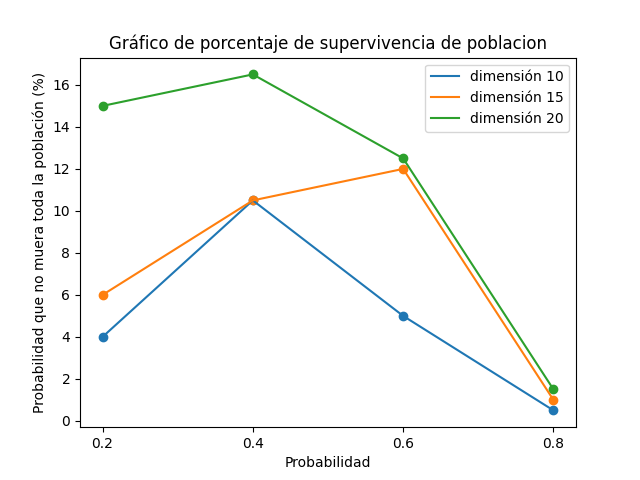
\includegraphics[width=200mm]{Figure_1.png}
    \caption{Diagrama puntos y líneas con dimensiones de 10, 15 y 20 con 200 replicas.}
    \label{figure}
\end{figure}

\section{Mediciones}

Para este caso se utilizaron 200 réplicas en lugar de 30 réplicas, para poder visualizar mejor el comportamiento de las dimensiones.

\begin{table}
    \centering
    \caption{Mediciones para la probabilidad en las dimensiones de: 10, 15 y 20}
    \begin{tabular}{|c|c|c|c||c|c||c|c|c|c||c|c|}
    \hline
       Dimensión & Probabilidad & Muertes & Réplicas & Vivos & Réplicas & Vpp\\
       \hline\hline
        10 & 0.2 & 30 & 192 & 30 & 8 & 4.0\\
        \hline
         & 0.4 & 30 & 179 & 30 & 21 & 5.5\\
        \hline
         & 0.6 & 30 & 190 & 30 & 10 & 3.0\\
        \hline
        & 0.8 & 30 & 199 & 30 & 1 & 0\\
        \hline
        15 & 0.2 & 30 & 188 & 30 & 12 & 6.5\\
        \hline
         & 0.4 & 30 & 179 & 30 & 21 & 11.5\\
        \hline
         & 0.6 & 30 & 176 & 30 & 24 & 6.0\\
        \hline
        & 0.8 & 30 & 198 & 30 & 2 & 0.5\\
        \hline
        20 & 0.2 & 30 & 170 & 30 & 30 & 13.5\\
        \hline
         & 0.4 & 30 & 167 & 30 & 33 & 13.5\\
        \hline
         & 0.6 & 30 & 175 & 30 & 25 & 16.5\\
        \hline
        & 0.8 & 30 & 197 & 30 & 3 & 2.0\\
        \hline
        
    \end{tabular}
    \label{medir_R}
\end{table}




\newpage
\section{Conclusion}

Se realizó la tarea 2 con éxito para obtener la probabilidad que se utilizó patra este caso de 200 réplicas ya que se puede representar mejor el diagrama.


\bibliography{simulacion}
\bibliographystyle{plain}


\end{document}
